\documentclass[letterpaper, 10pt, openany]{memoir}

\usepackage{graphicx}
\usepackage{verse}
\graphicspath{{./images/}}

% Title
\pretitle{\begin{center}\bfseries}
\title{\Huge{How to Tell the Birds from the Flowers.\\}
\huge{A Manual of Flornithology for Beginners.}}
\posttitle{\end{center}
\includegraphics[width=1\textwidth]{f-p-i.png}}
\author{Verses and Illustrations\\
By Robert Williams Wood}
\date{}

%Chapter
\makechapterstyle{custom} {
	\renewcommand{\thechapter}{}
	\renewcommand{\chapterheadstart}{}
	\renewcommand{\printchaptername}[1]{##1}
	\renewcommand{\chapternamenum}{}
	\renewcommand{\printchapternum}{}
	\renewcommand{\afterchapternum}{}
	\renewcommand{\printchaptertitle}[1]{}
	\renewcommand{\afterchaptertitle}{}
}
\chapterstyle{custom}

%Table of Contents
\renewcommand\printtoctitle[1]{\section*{#1}}
\renewcommand\aftertoctitle{}

\begin{document}
\raggedright
\frontmatter
\maketitle
\vspace{\onelineskip}
\begin{center}
Published by Paul Elder and Company

San Francisco and New York.
\end{center}

\clearpage
\thispagestyle{plain}
\begin{figure}[b]
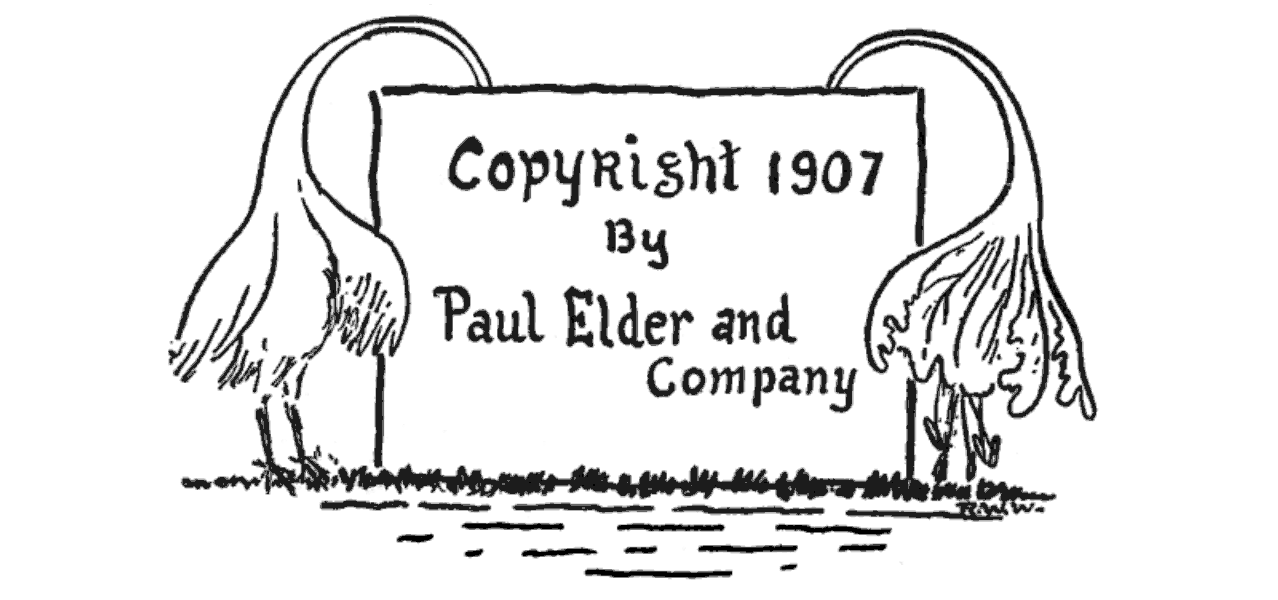
\includegraphics[width=1\textwidth]{f-p-ii.png}
\end{figure}

\clearpage
\thispagestyle{plain}
\tableofcontents*

\mainmatter
\chapter{The Bird. The Birdock.}
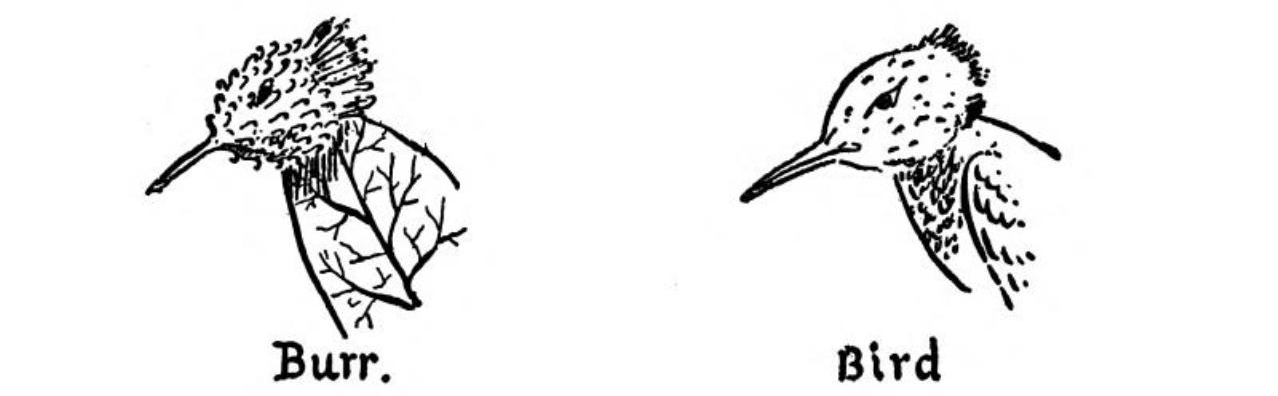
\includegraphics[width=1\textwidth]{f-p01a.png}
\begin{center}
\large{\textbf{The Bird and the Burdock.}}
\end{center}
\vspace{\onelineskip}
\begin{verse}\huge
Who \underline{is} there who has never heard,\\
About the Burdock and the Bird?\\
And yet how \underline{very} \underline{very} few,\\
Discriminate between the two,\\
While even Mr. Burbank can't\\
Transform a Bird into a Plant!\\
\end{verse}
\vspace{\onelineskip}

\includegraphics[width=1\textwidth]{f-p01b.png}

\chapter{The Clover. The Plover.}
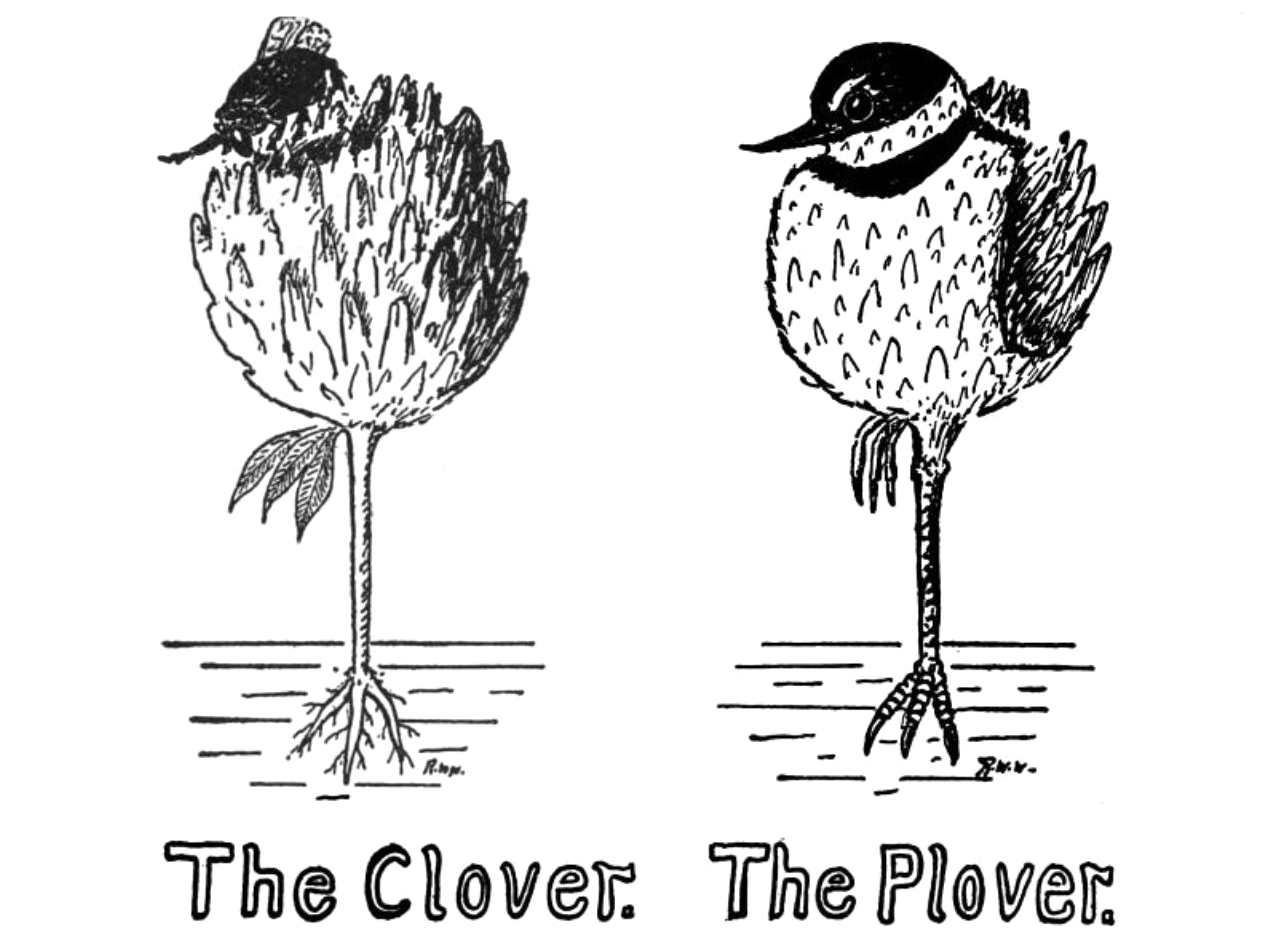
\includegraphics[width=1\textwidth]{f-p02.png}
\vspace{\onelineskip}
\begin{verse}\huge
The Plover and the Clover can be told apart with ease,\\
By paying close attention to the habits of the Bees,\\
For ento-molo-gists aver, the Bee can be in Clover,\\
While ety-molo-gists concur, there is no B in Plover.\\
\end{verse}
\vspace{\onelineskip}

\chapter{The Crow. The Crocus.}
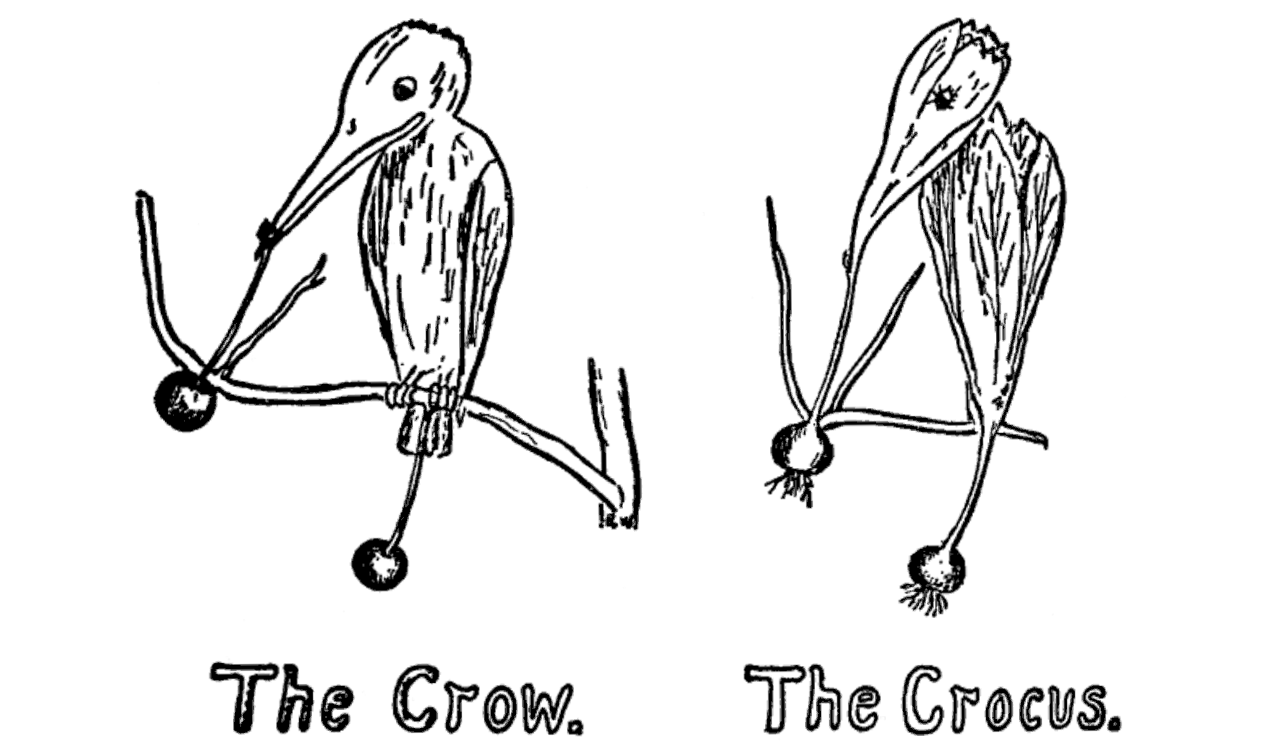
\includegraphics[width=1\textwidth]{f-p03.png}
\vspace{\onelineskip}
\begin{verse}\huge
Some are unable, as you know,\\
To tell the Crocus from the Crow;\\
The reason why is just because\\
They are not versed in Nature's laws.\\
The noisy, cawing Crows all come,\\
Obedient to the Cro'custom,\\
A large Crow Caw-cus to convoke.\\
You \underline{never} hear the Crocus croak!\\
\end{verse}
\vspace{\onelineskip}

\chapter{The Rue. The Rooster}
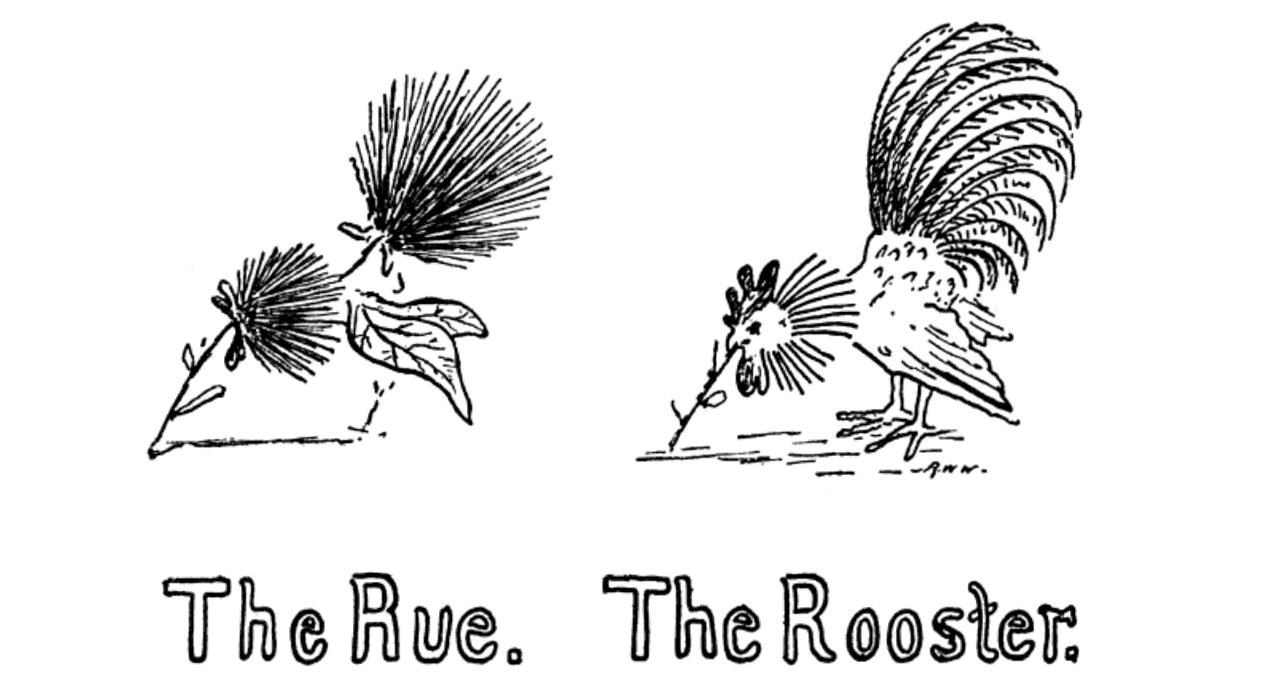
\includegraphics[width=1\textwidth]{f-p04.png}
\vspace{\onelineskip}
\begin{verse}\huge
Of Rooster the rudiment clearly is "\underline{Roo}",\\
And the bird from the plant very probably grew.\\
You can easily tell them apart without fail,\\
By merely observing the Rue lacks de-tail.\\
\end{verse}
\vspace{\onelineskip}

\chapter{The Parrot. The Carrot}
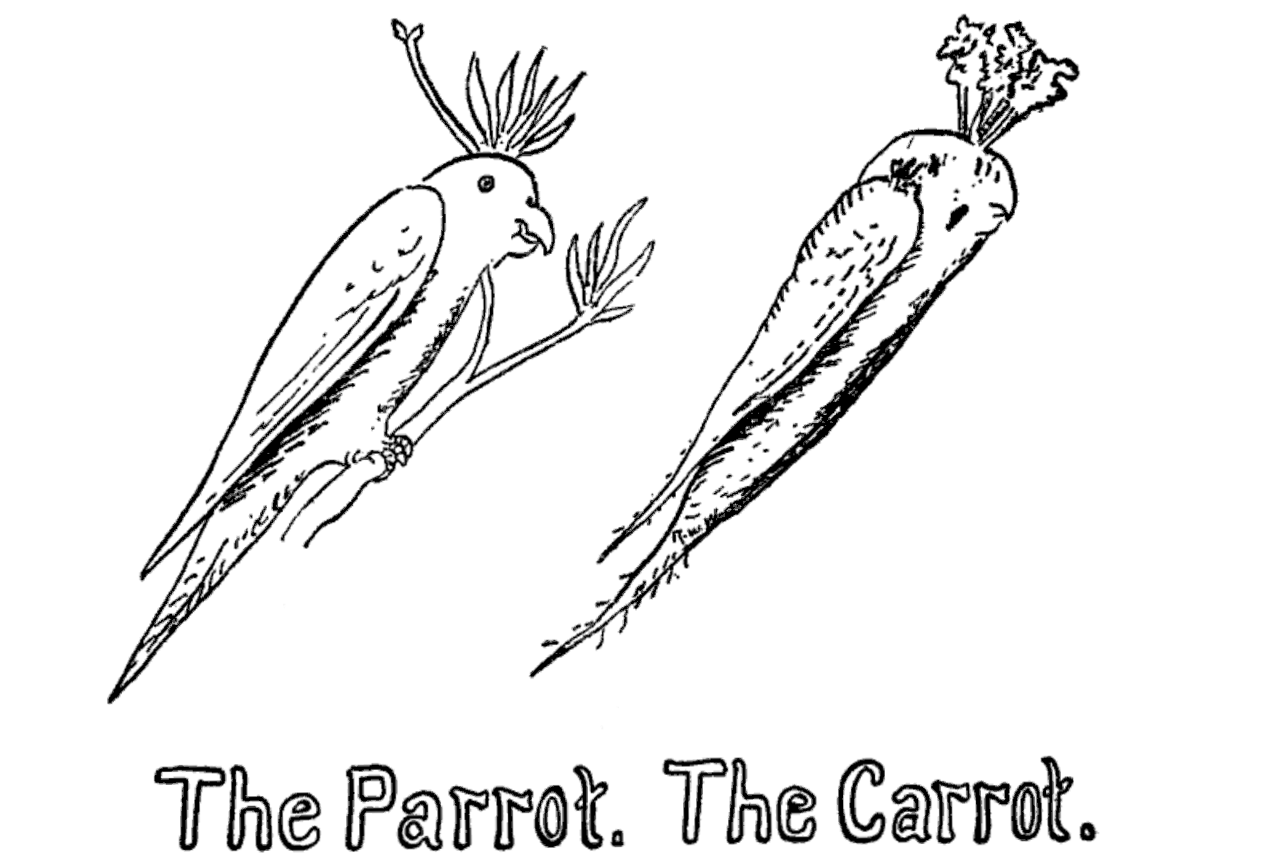
\includegraphics[width=1\textwidth]{f-p05.png}
\vspace{\onelineskip}
\begin{verse}\huge
The Parrot and the Carrot we may easily confound,\\
They're very much alike in looks and similar in sound,\\
We recognize the Parrot by his clear articulation,\\
For Carrots are unable to engage in conversation.\\
\end{verse}
\vspace{\onelineskip}

\chapter{The Pea. The Pewee}
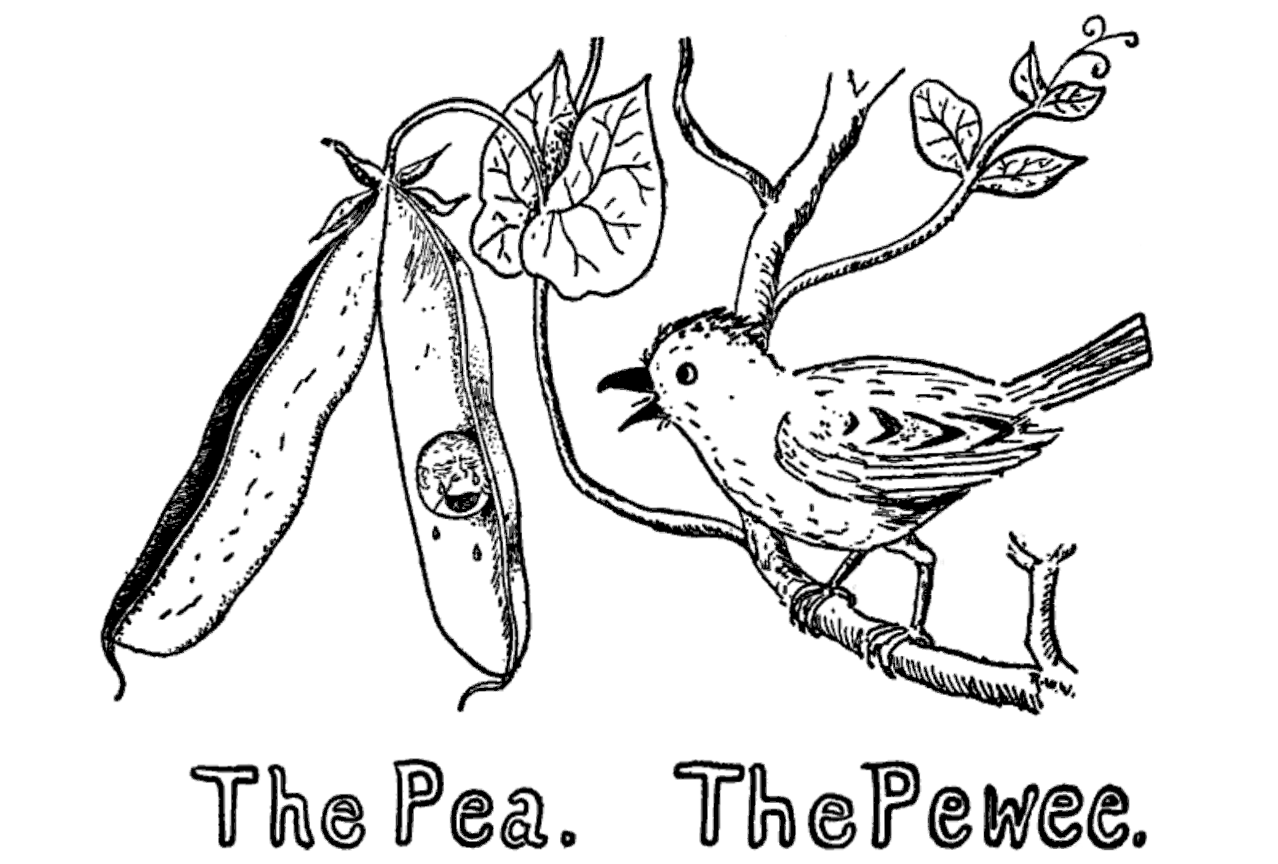
\includegraphics[width=1\textwidth]{f-p06.png}
\vspace{\onelineskip}
\begin{verse}\huge
To tell the Pewee from the Pea,\\
Requires great per-spi-cac-ity.\\
Here in the pod we see the Pea,\\
While perched close by is the Pewee;\\
The Pea he hears the Pewee peep,\\
While Pewee sees the wee Pea weep,\\
There'll be but little time to see,\\
How Pewee differs from the Pea.\\
\end{verse}
\vspace{\onelineskip}

\chapter{The Pelican. The Panicle}
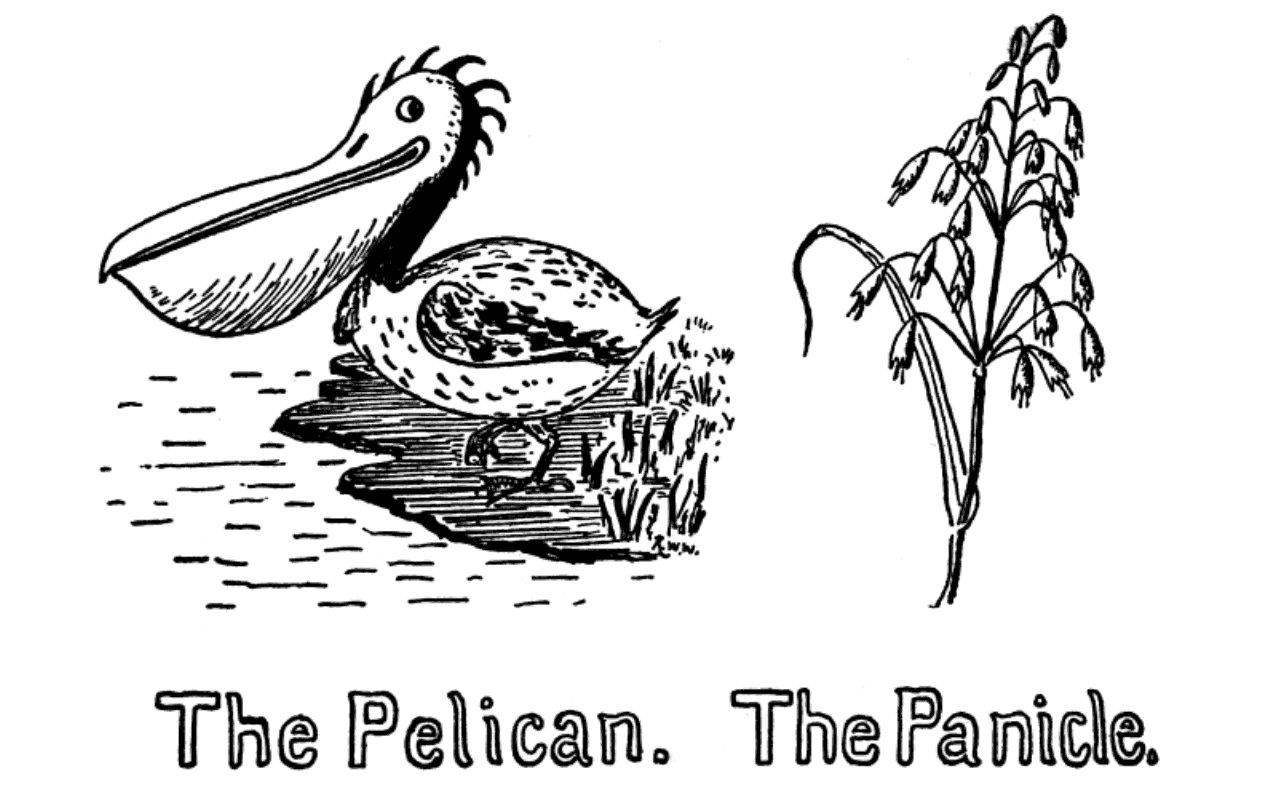
\includegraphics[width=1\textwidth]{f-p07.png}
\vspace{\onelineskip}
\begin{verse}\huge
The Panicle and Pelican\\
Have often been confused;\\
The letters which spell Pelican\\
In Panicle are used.\\
You never need confound the two,\\
There are many ways of telling:\\
The simplest thing that one can do,\\
Is to observe the spelling.\\
\end{verse}
\vspace{\onelineskip}

\chapter{The Hen. The Lichen}
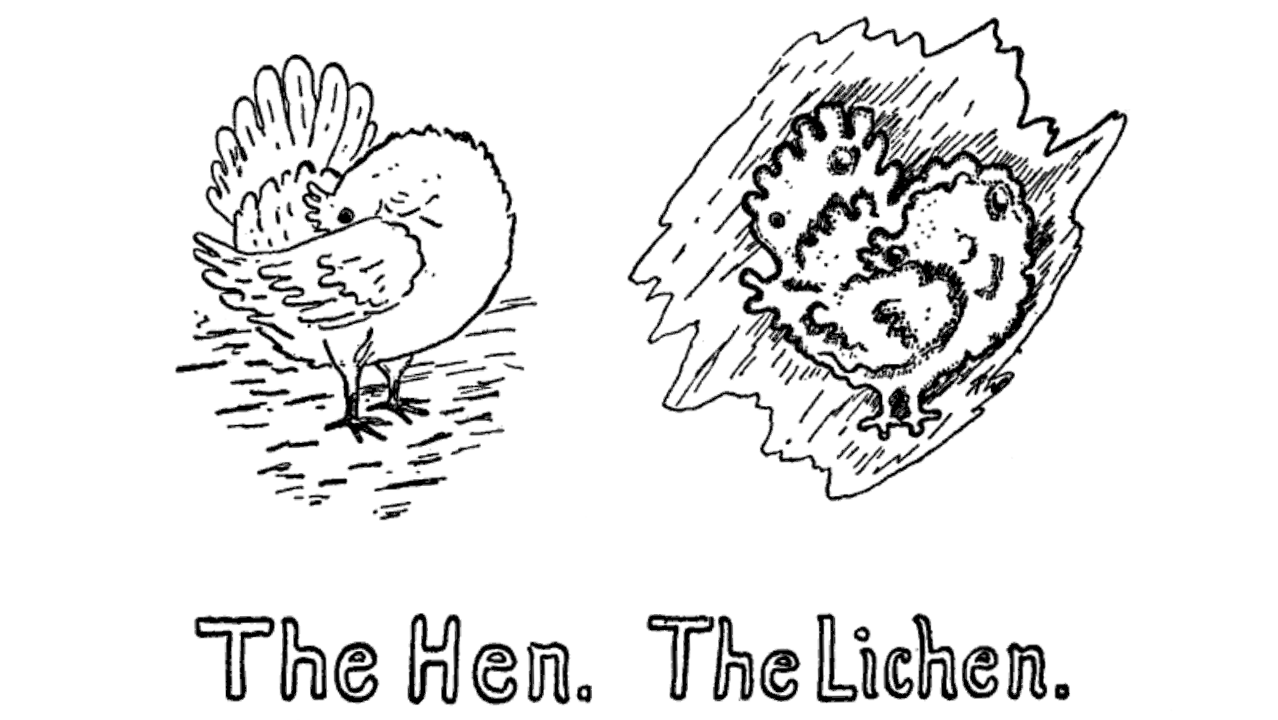
\includegraphics[width=1\textwidth]{f-p08.png}
\vspace{\onelineskip}
\begin{verse}\huge
The Lichens lie on rocks and bark,\\
They look somewhat like Hens:\\
Hens \underline{lay}, they \underline{lie}, we may remark,\\
A difference of tense.\\
\end{verse}
\vspace{\onelineskip}

\chapter{The Hawk. The Hollyhock}
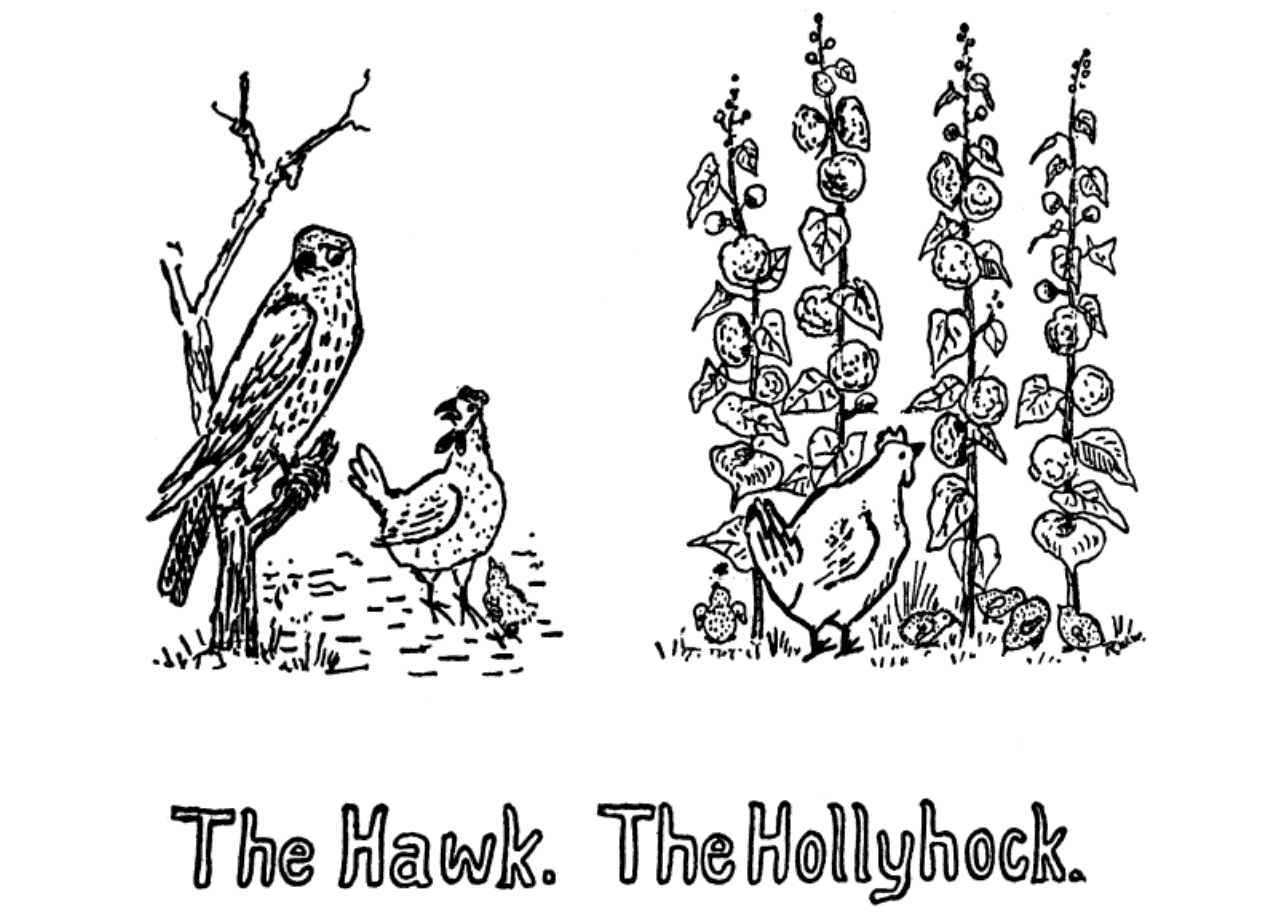
\includegraphics[width=1\textwidth]{f-p09.png}
\vspace{\onelineskip}
\begin{verse}\huge
To recognize this Bird-of-Prey,\\
The broody Hen you should survey:\\
She takes her Chicks on daily walks,\\
Among the neighboring Hollyhocks,\\
While with the Hawk association,\\
Is quite beyond her toleration.\\
\end{verse}
\vspace{\onelineskip}

\chapter{The Cow Bird. The Cowslip}
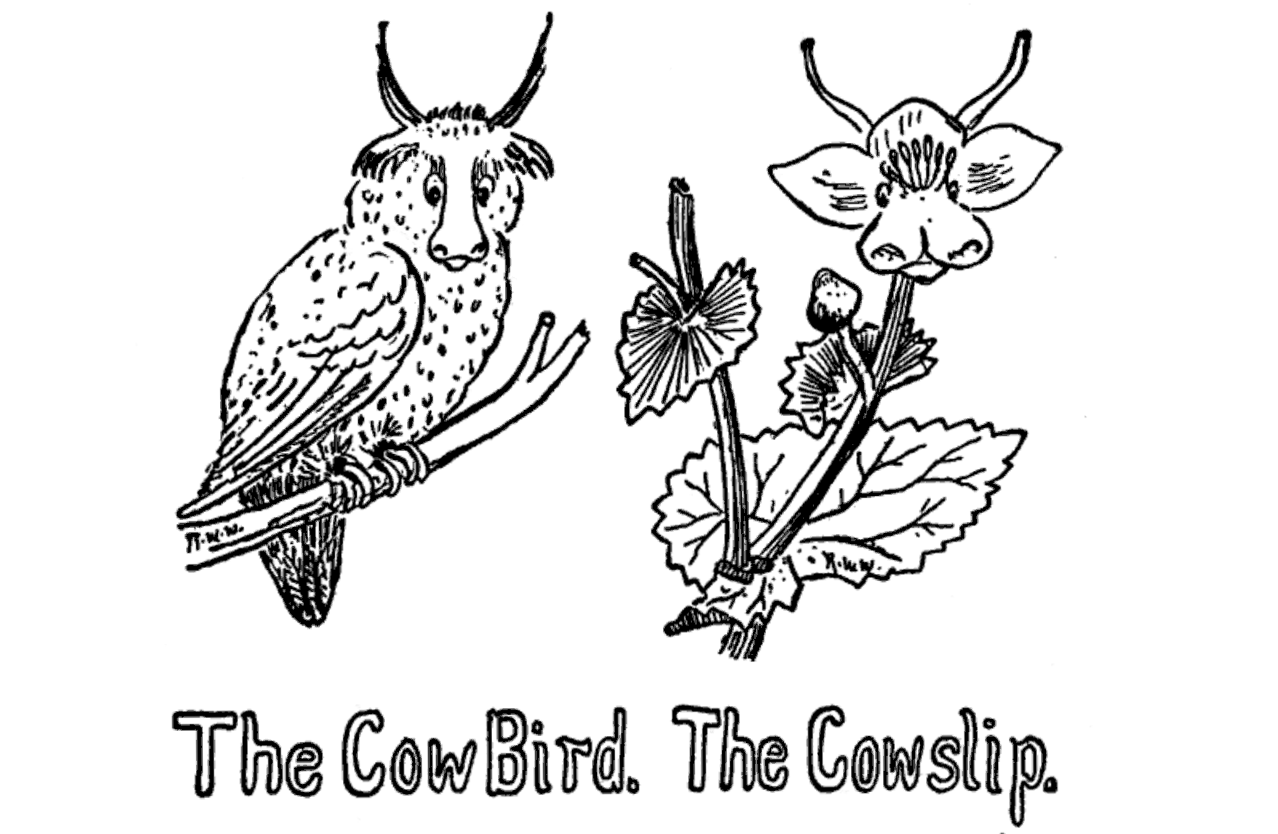
\includegraphics[width=1\textwidth]{f-p10.png}
\vspace{\onelineskip}
\begin{verse}\huge
Growing in mires, in gold attired,\\
The Cowslip has been much admired,\\
Although its proper name, we're told,\\
Is really the Marsh Marigold:\\
The Cow Bird picture, I suspect,\\
Is absolutely incorrect,\\
We make such errors now and then,\\
A sort of cow slip of the pen.\\
\end{verse}
\vspace{\onelineskip}

\chapter{The Sparrer. Asparagus.}
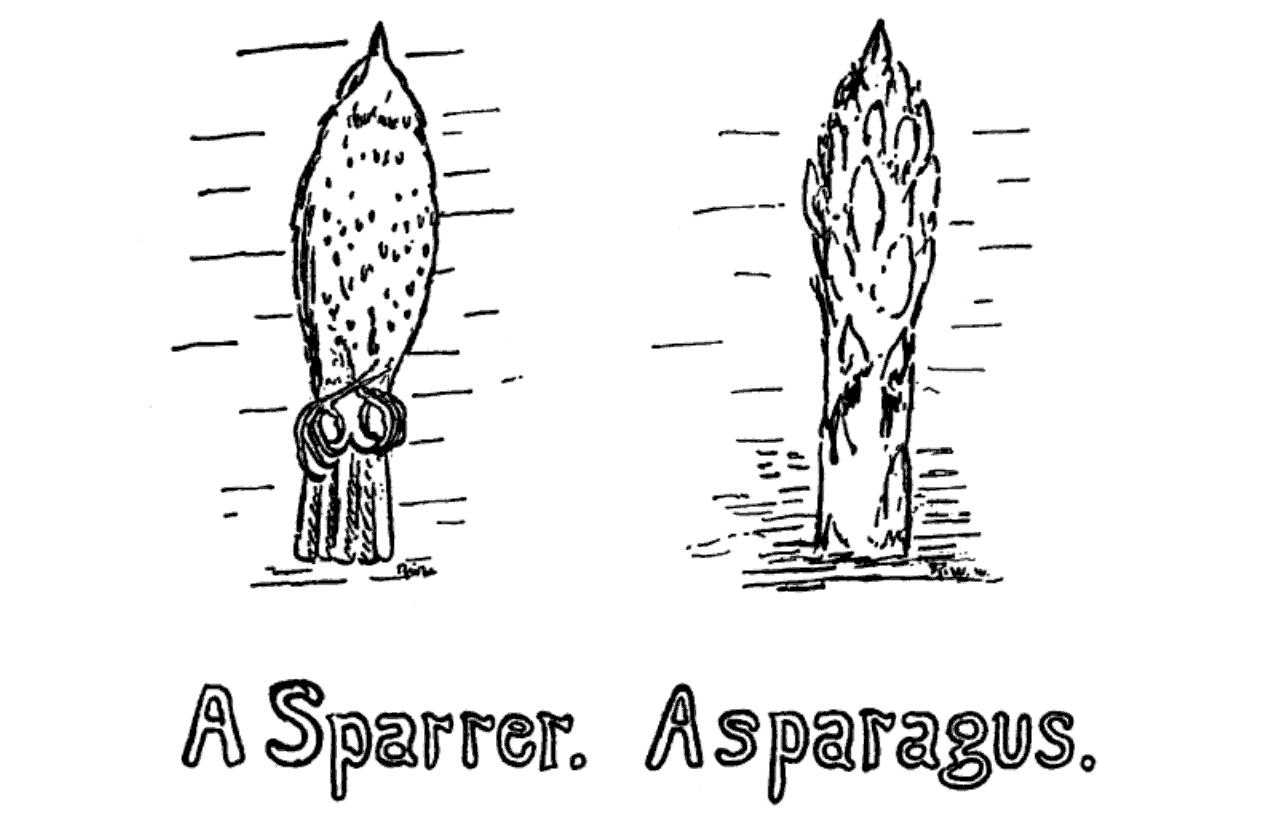
\includegraphics[width=1\textwidth]{f-p11.png}
\vspace{\onelineskip}
\begin{verse}\huge
The Sparrow, from flying, is quite out of breath,\\
In fact he has worked himself almost to death,\\
While the lazy Asparagus, so it is said,\\
Spends all of his time in the 'sparagus bed.\\
\end{verse}

\chapter{The Tern. The Turnip.}
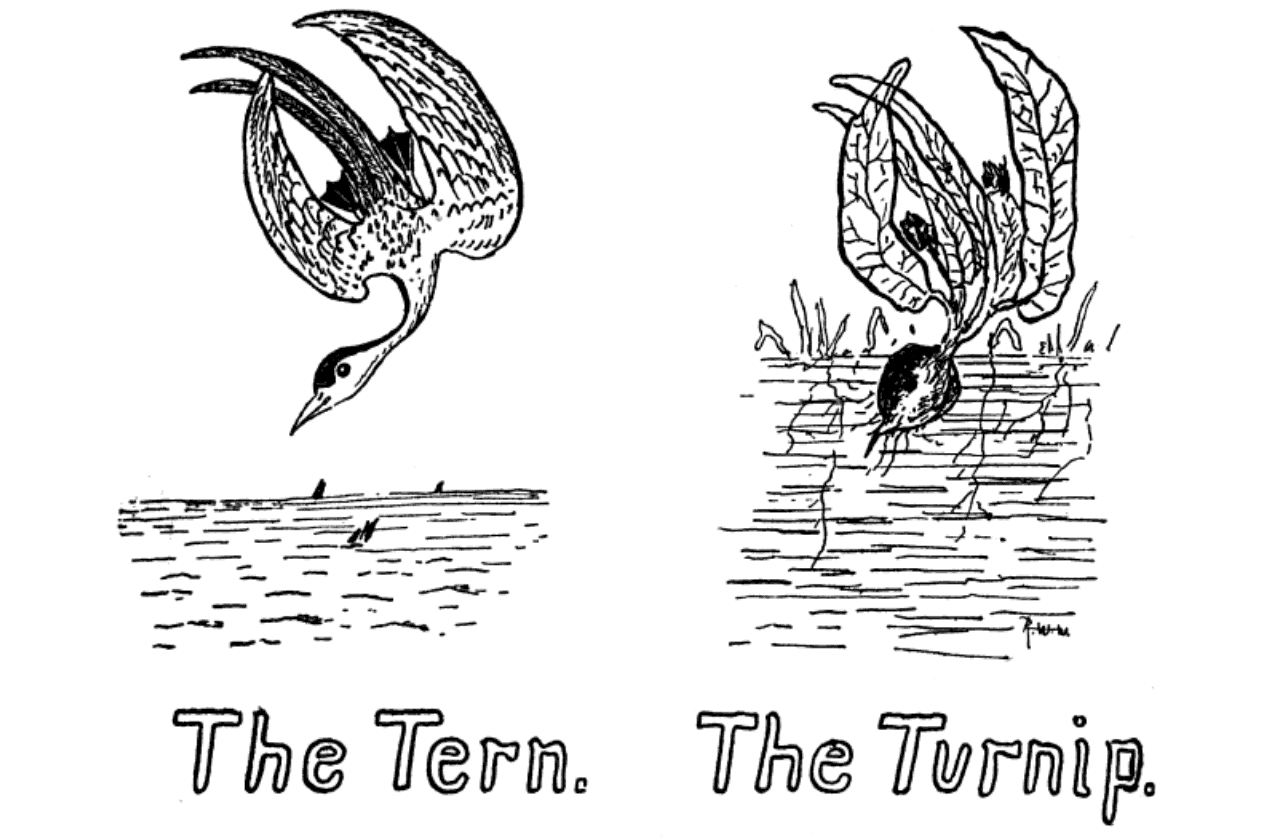
\includegraphics[width=1\textwidth]{f-p12.png}
\vspace{\onelineskip}
\begin{verse}\huge
To tell the Turnip from the Tern,\\
A thing which everyone should learn,\\
Observe the Tern up in the air,\\
See how he turns,--and now compare\\
Him with this inert vegetable,\\
Who thus to turn is quite unable,\\
For he is rooted to the spot,\\
\newpage
While as we see the Tern is not:\\
He is not always doomed to be\\
Thus bound to earth e-\underline{tern}-ally,\\
For "Cooked to a turn" may be inferred,\\
To change the Turnip to the Bird.\\
\end{verse}

\vspace{\onelineskip}
\vspace{\onelineskip}
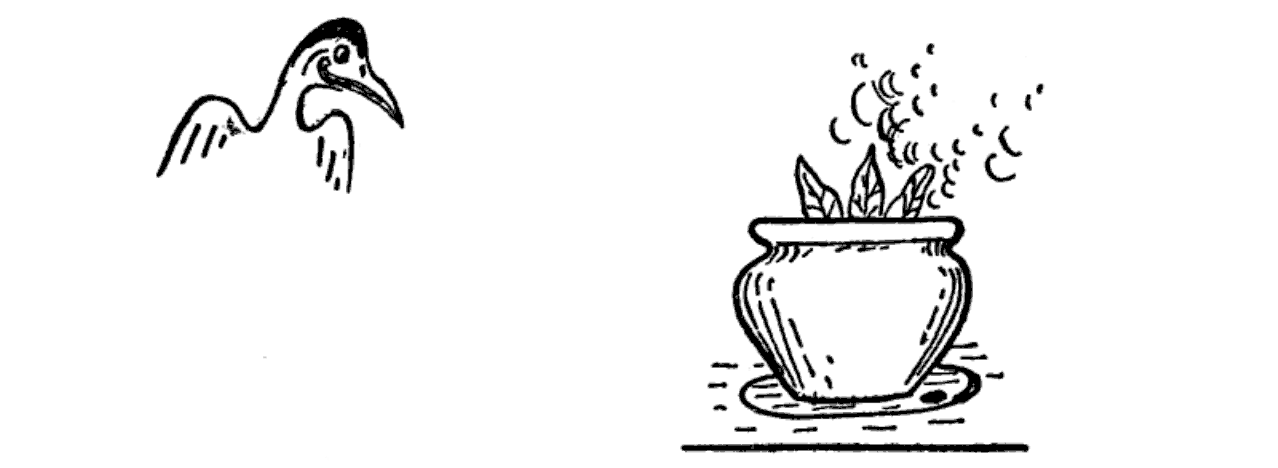
\includegraphics[width=1\textwidth]{f-p13.png}\\
\vspace{\onelineskip}
\vspace{\onelineskip}

\begin{verse}\huge
Observe the Turnip in the pot.\\
The Tern is glad that he is not!\\
\end{verse}

\chapter{The Ole Gander. The Oleander.}
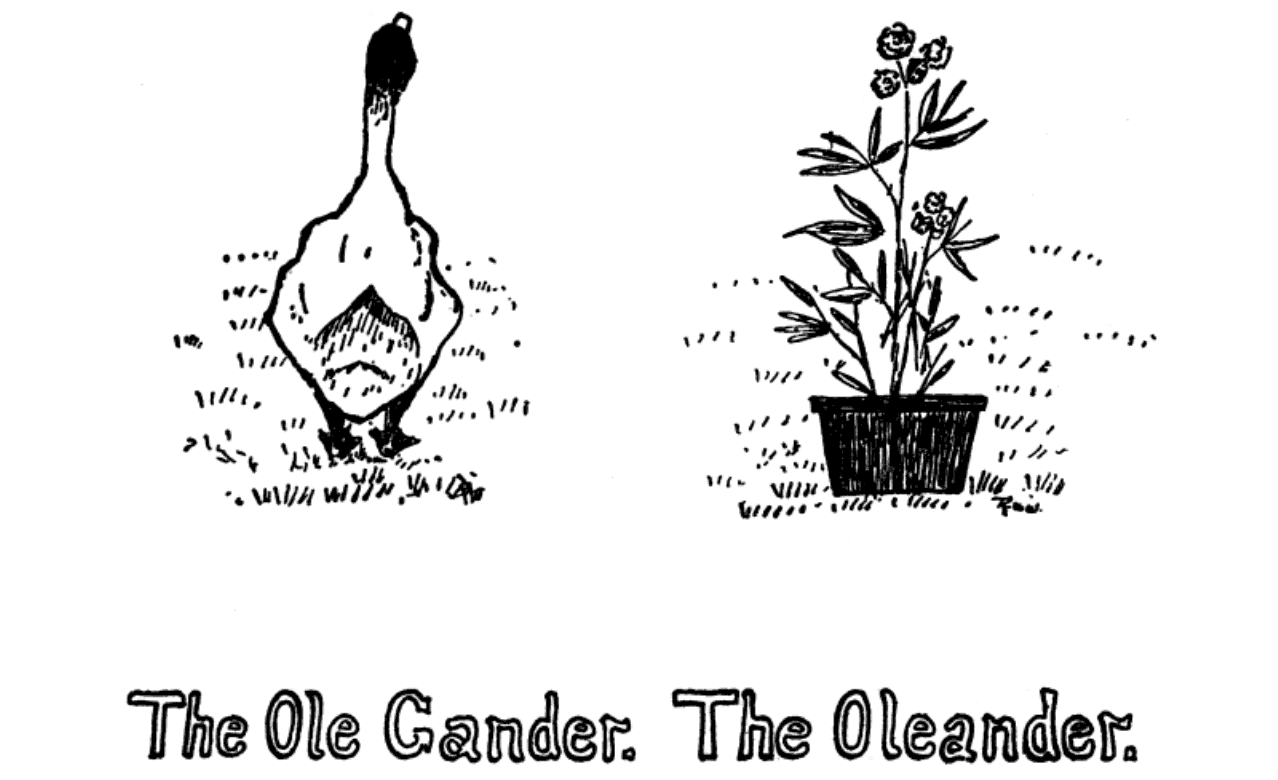
\includegraphics[width=1\textwidth]{f-p14.png}
\vspace{\onelineskip}
\begin{verse}\huge
The Gander loves to promenade,\\
Around the farmer's poultry-yard,\\
While, as we see, the Oleander\\
Is quite unable to meander\\
\end{verse}

\chapter{The Bule Mountain Lory. The Blue Morning Glory.}
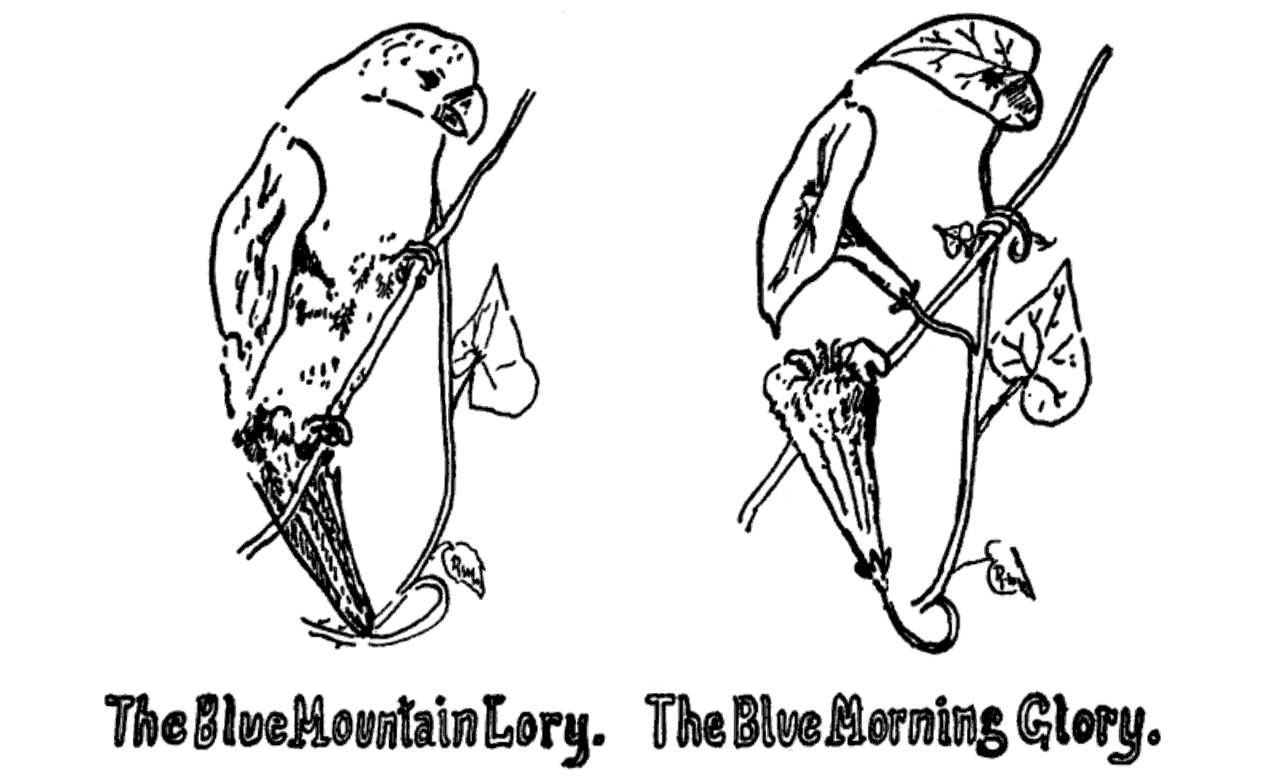
\includegraphics[width=1\textwidth]{f-p15.png}
\vspace{\onelineskip}
\begin{verse}\huge
The Blue Mountain Lory spends most of his time\\
In climbing about in a tropical clime;\\
We therefore our efforts need only confine,\\
To minutely observing the climb of the Vine.\\
\end{verse}

\chapter{The Quail. The Kale.}
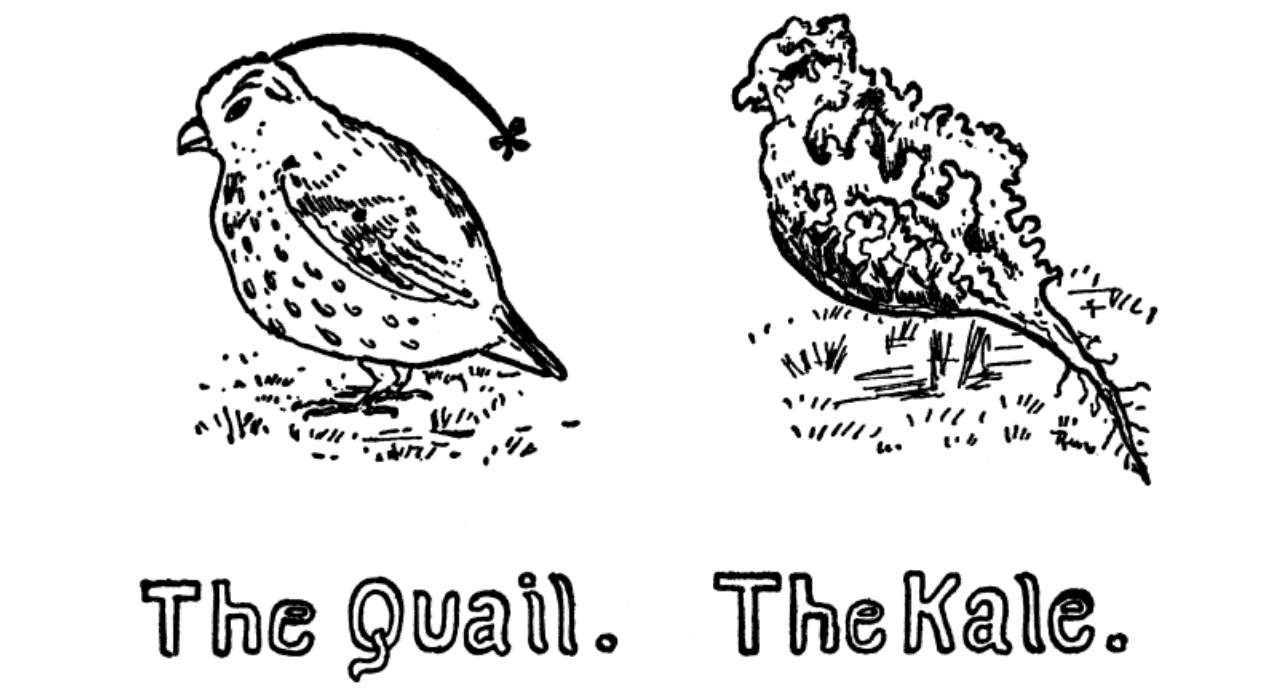
\includegraphics[width=1\textwidth]{f-p16.png}
\vspace{\onelineskip}
\begin{verse}\huge
The California Quail is said\\
To have a tail upon his head!\\
While contrary-wise we style the Kale,\\
A cabbage head upon a tail.\\
It is not hard to tell the two,\\
The Quail commences with a queue.\\
\end{verse}

\chapter{The Pecan. The Toucan.}
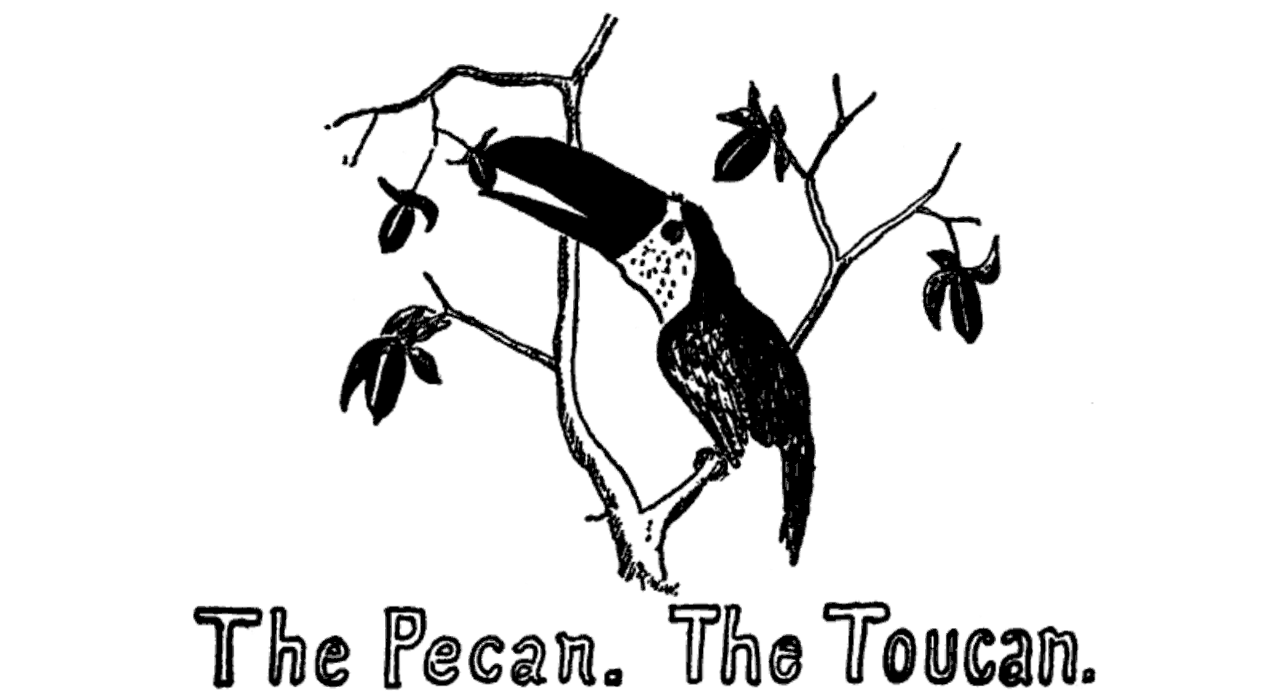
\includegraphics[width=1\textwidth]{f-p17.png}
\vspace{\onelineskip}
\begin{verse}\huge
Very few can\\
Tell the Toucan\\
From the Pecan--\\
Here's a new plan:\\
To take the Toucan from the tree,\\
Requires im-mense agil-i-ty,\\
While \underline{any one} can pick with ease\\
The Pecans from the Pecan trees:\\
It's such an easy thing to do,\\
That even the Toucan he can too.\\
\end{verse}

\chapter{The Auk. The Orchid.}
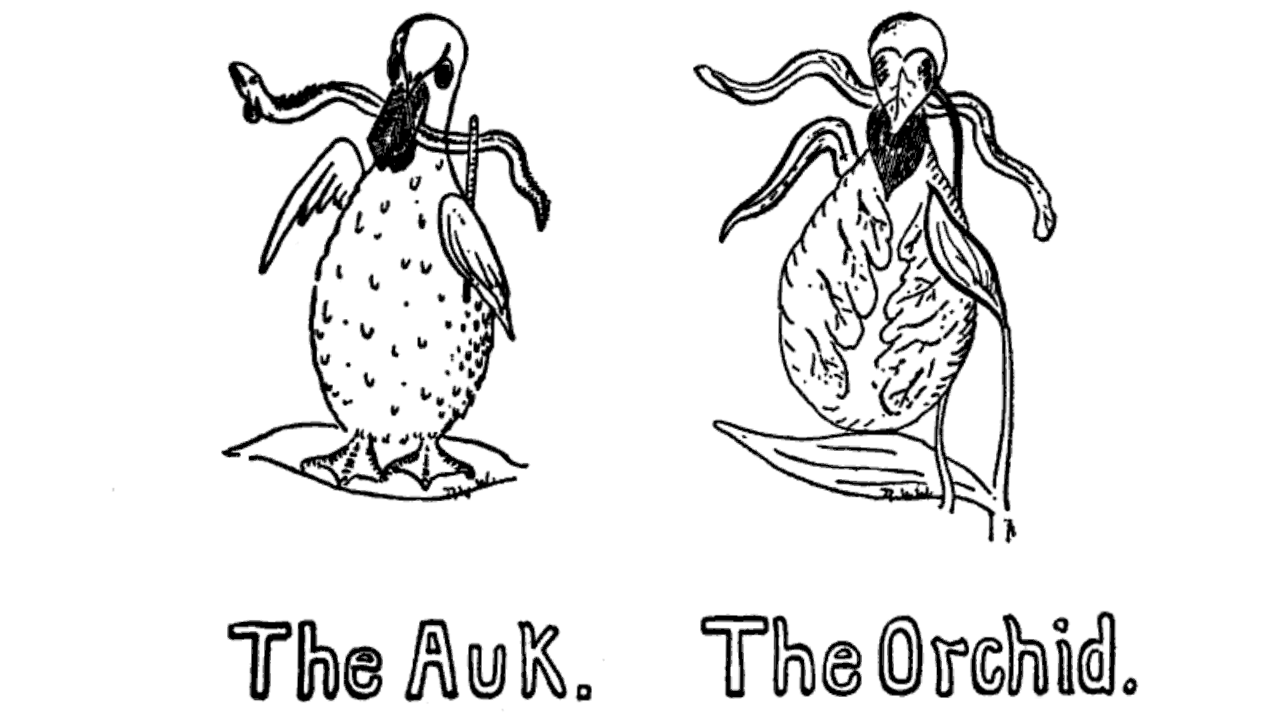
\includegraphics[width=1\textwidth]{f-p18.png}
\vspace{\onelineskip}
\begin{verse}\huge
We seldom meet, when out to walk,\\
Either the Orchid or the Auk;\\
The Auk indeed is only known\\
To dwellers in the Auktic zone,\\
While Orchids can be found in legions,\\
Within the equatorial regions.\\
The graceful Orchid on its stalk,\\
Resembles so the aukward Auk;\\
\newpage
'Tis plain we must some means discover,\\
To tell the two from one another:\\
The obvious difference, to be sure,\\
Is merely one of temperature.\\
\end{verse}

\vspace{\onelineskip}
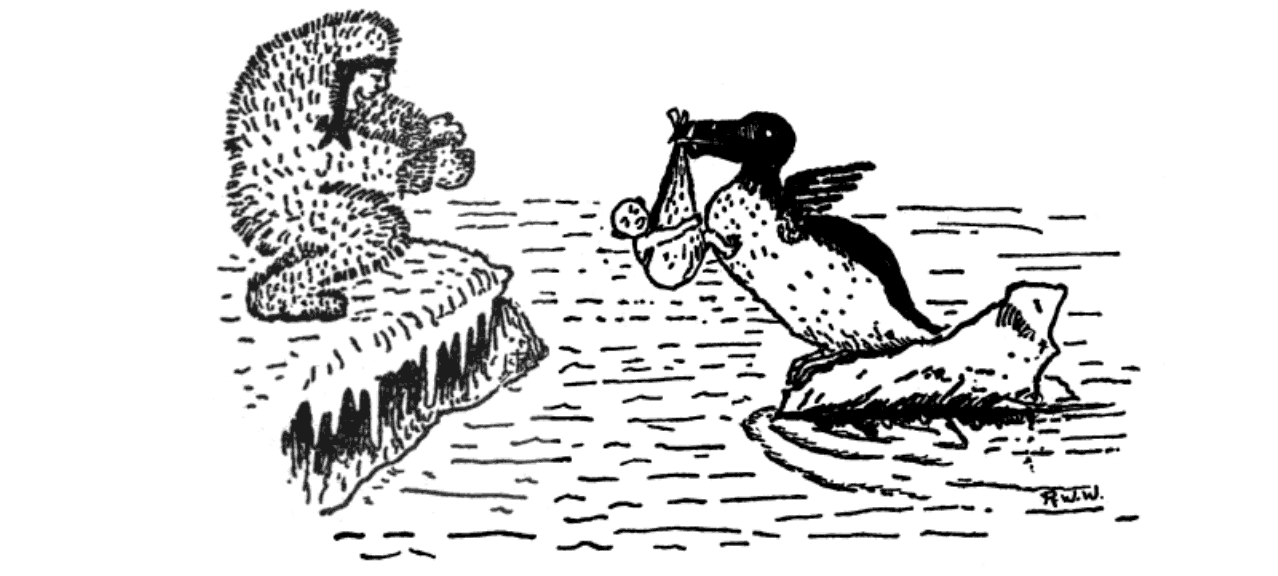
\includegraphics[width=1\textwidth]{f-p19.png}
\vspace{\onelineskip}

\begin{verse}\huge
For Eskimos, perhaps, the Auk\\
Performs the duties of the Stork.\\
\end{verse}

\chapter{The Cat-bird. The Cat-nip.}
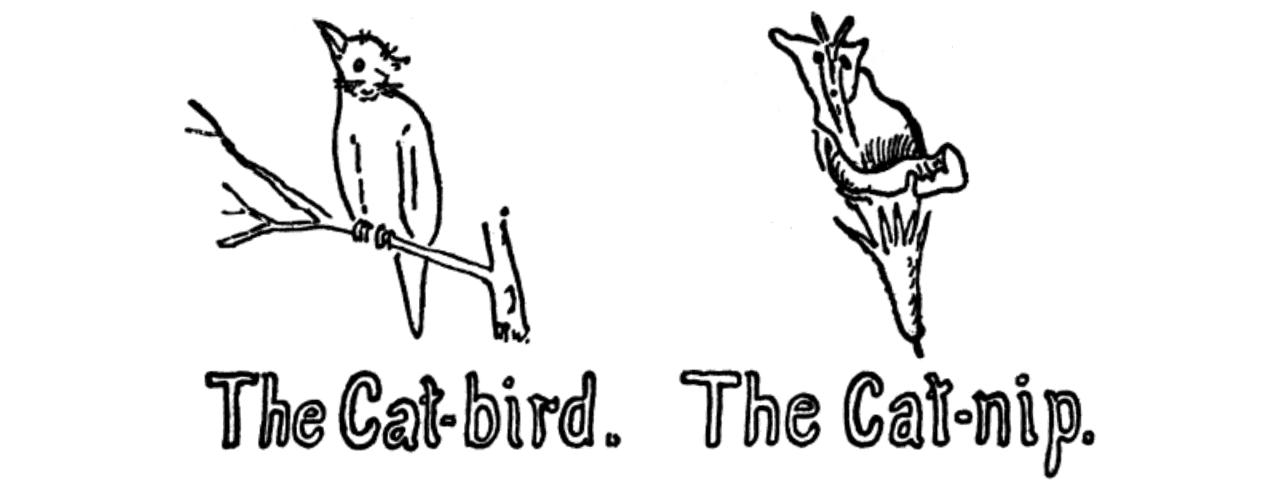
\includegraphics[width=1\textwidth]{f-p20a.png}
\vspace{\onelineskip}
\begin{verse}\huge
The Cat-bird's call resembles that,\\
Emitted by the Pussy Cat,\\
While Cat-nip, growing by the wall,\\
Is never known to caterwaul:\\
Its odor though attracts the Kits,\\
And throws them in Catniption fits.\\
\end{verse}
\vspace{\onelineskip}
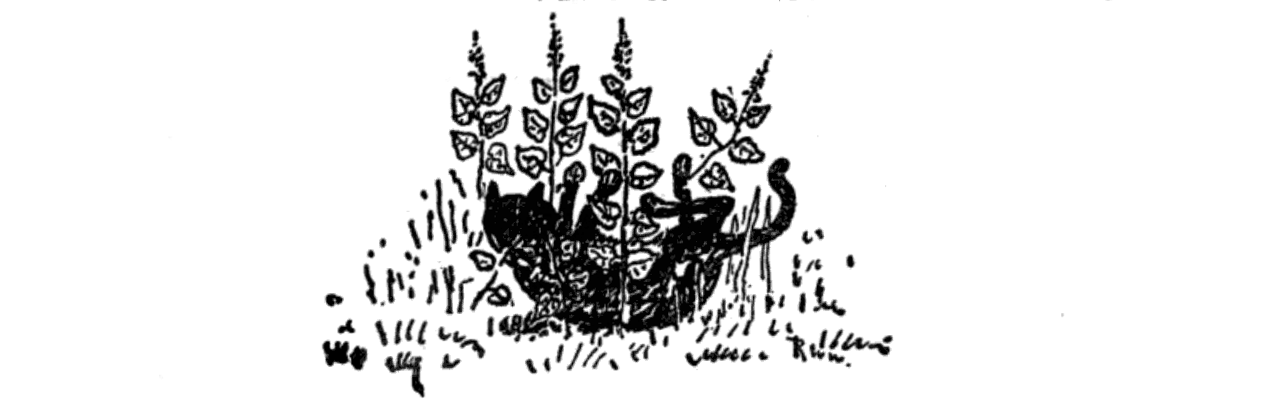
\includegraphics[width=1\textwidth]{f-p20b.png}

\chapter{The Ibis. The 'Ibiscus.}
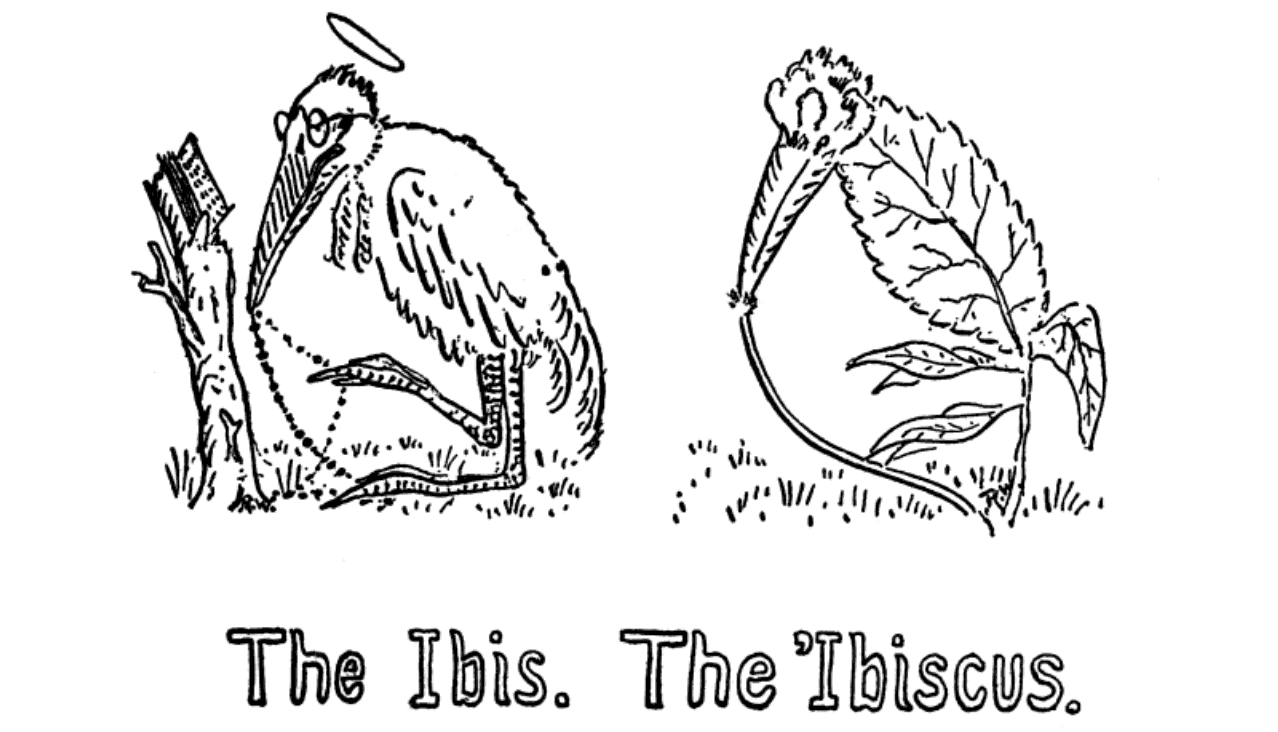
\includegraphics[width=1\textwidth]{f-p21.png}
\vspace{\onelineskip}
\begin{verse}\huge
The sacred Ibis tells his beads,\\
And gravely from his prayer-book reads;\\
The Ibis therfore we may say,\\
Is classified a bird-of-prey.\\
'Ibiscus we have heard related,\\
The "Crimson-Eye" is designated;\\
Their difference is plain indeed,\\
The flower is red, the bird can read.\\
\end{verse}

\chapter{The Butter-ball. The Butter-cup.}
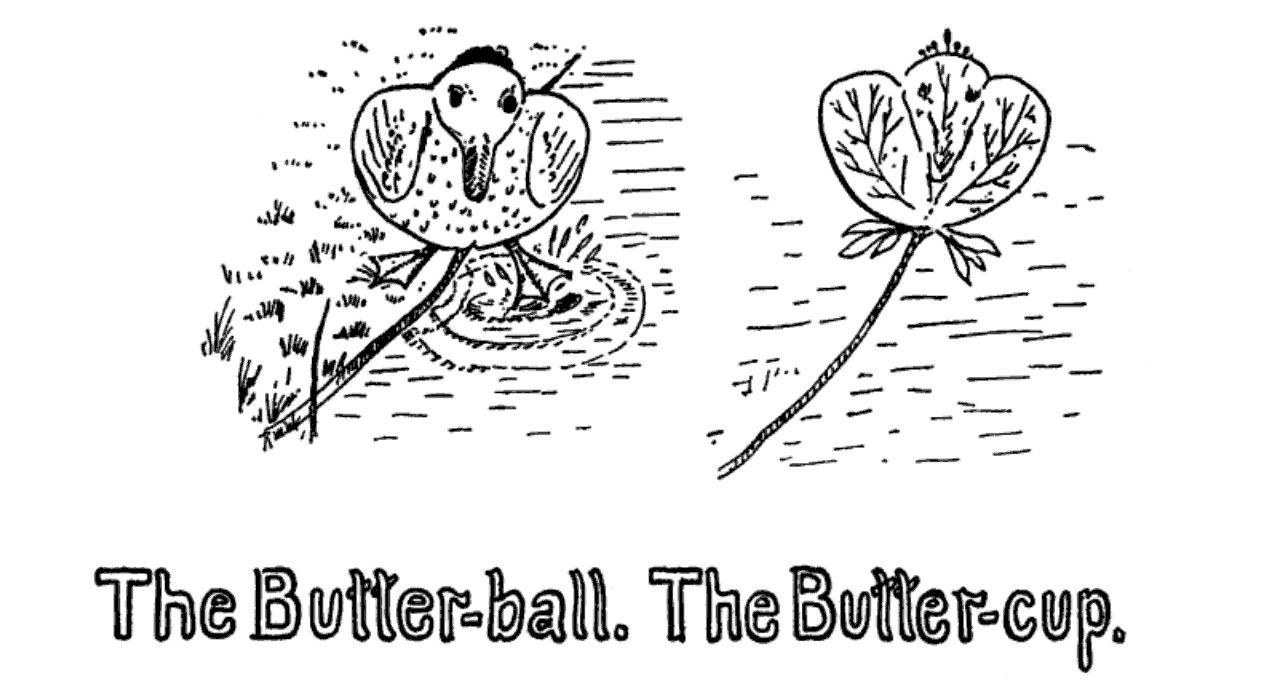
\includegraphics[width=1\textwidth]{f-p22a.png}
\vspace{\onelineskip}
\begin{verse}\huge
The little Butter-cup can sing,\\
From morn 'til night like anything:\\
The quacking of the Butter-ball,\\
Cannot be called a song at all.\\
We thus the flower may learn to know,\\
Its song is reproduced below.\\
\end{verse}
\vspace{\onelineskip}

\includegraphics[width=1\textwidth]{f-p22b.png}

\chapter{The Bay. The Jay.}
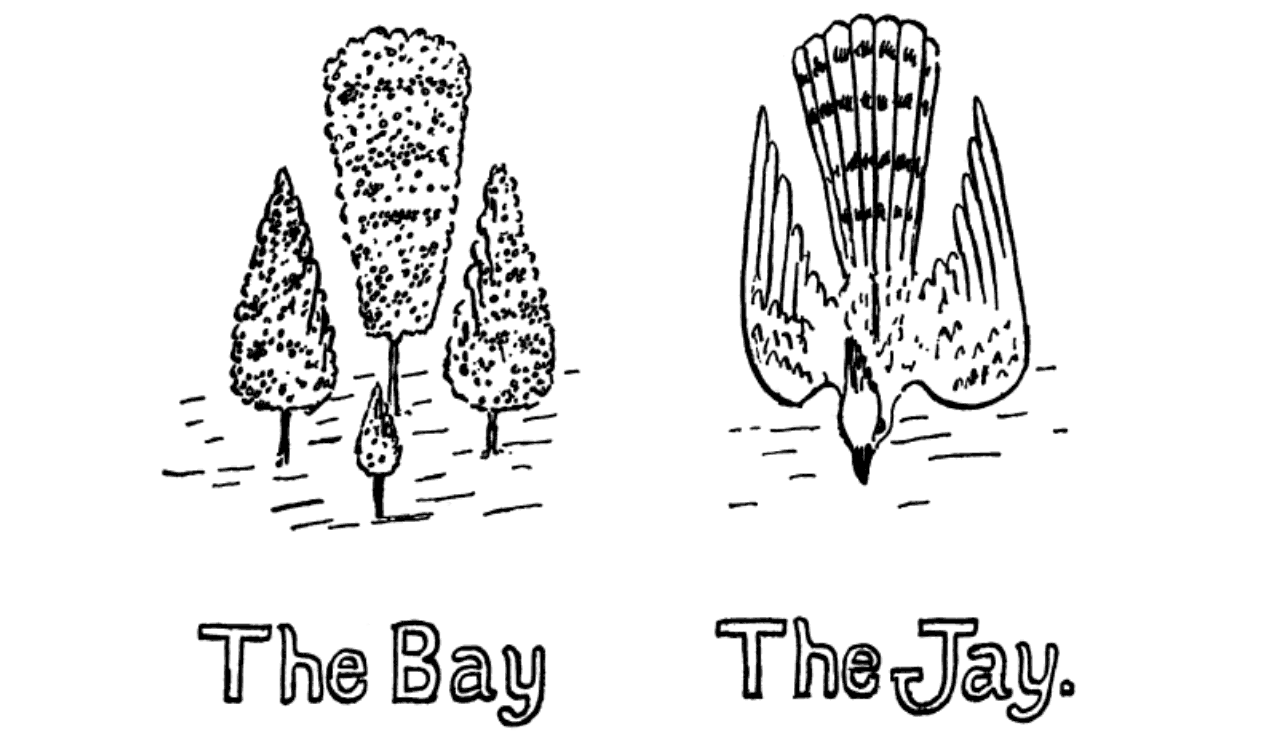
\includegraphics[width=1\textwidth]{f-p23.png}
\vspace{\onelineskip}
\begin{verse}\huge
The Blue-Jay, as we plainly see,\\
Resembles much the green Bay tree:\\
The difference between the two,\\
Is ob-vi-ous-ly one of hue.\\
Though this is not the only way,\\
To tell the Blue-Jay from the Bay.\\
\end{verse}

\chapter{The Pipe. The Snipe.}
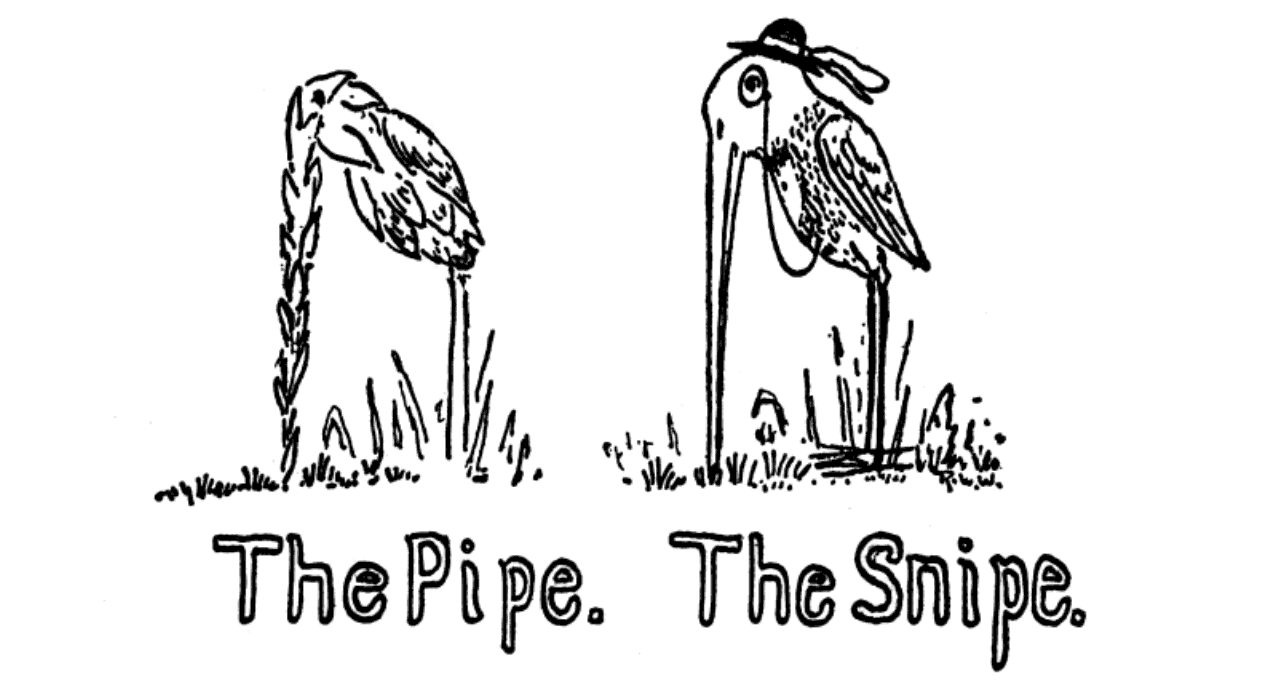
\includegraphics[width=1\textwidth]{f-p24a.png}
\vspace{\onelineskip}
\begin{verse}\huge
Observe the common Indian Pipe,\\
Likewise the high-bred English Snipe,\\
Who is distinguished, as we see,\\
By his superior pedigree.
\end{verse}
\vspace{\onelineskip}

\includegraphics[width=1\textwidth]{f-p24b.png}

\chapter{The Roc. The Shamrock.}
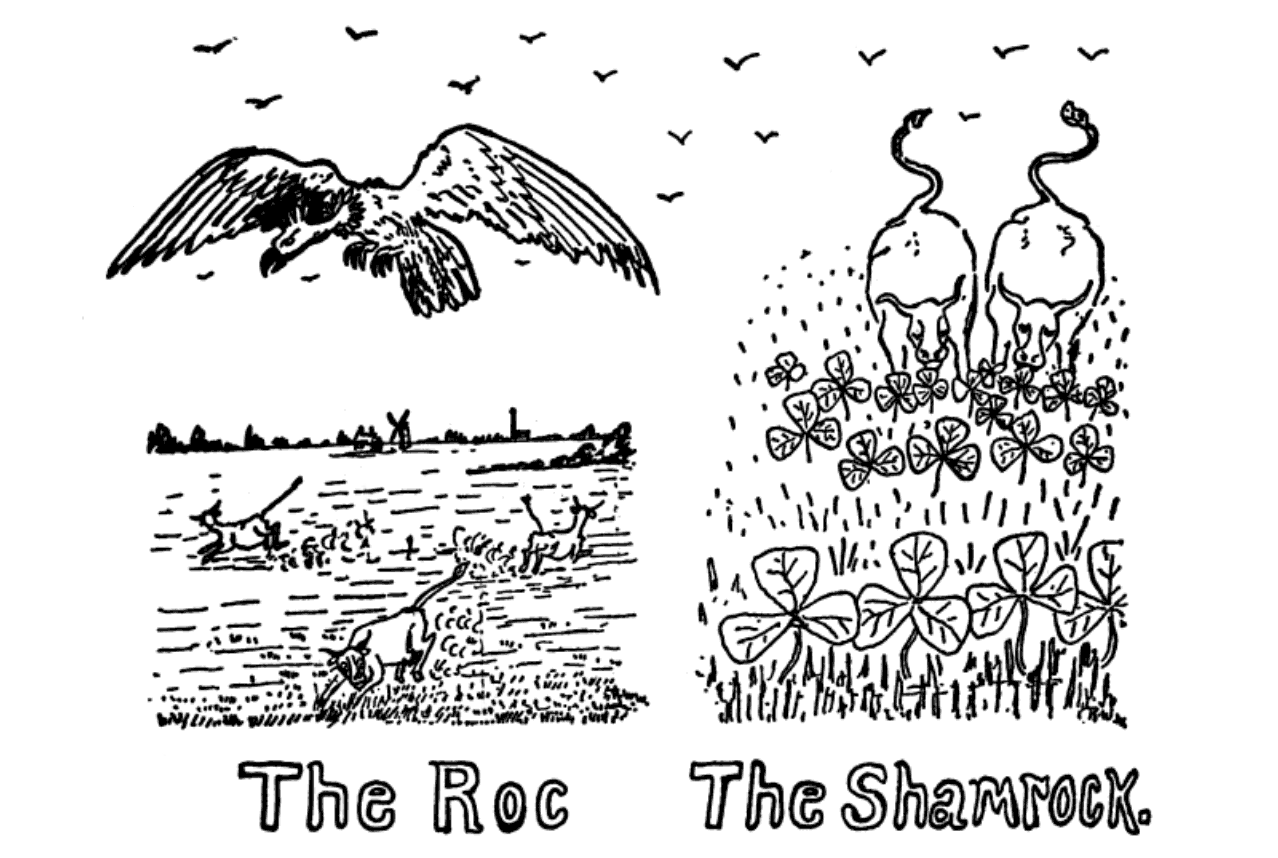
\includegraphics[width=1\textwidth]{f-p25.png}
\vspace{\onelineskip}
\begin{verse}\huge
Observe how peacefully the Cows\\
Among the little Shamrocks browse,\\
In contrast with their actions frantic\\
When they perceive the Roc gigantic;\\
We need but watch thei\textbf{r oc}cupation.\\
And seek no other explanation.\\
\end{verse}

\chapter{The Lark. The Larkspur.}
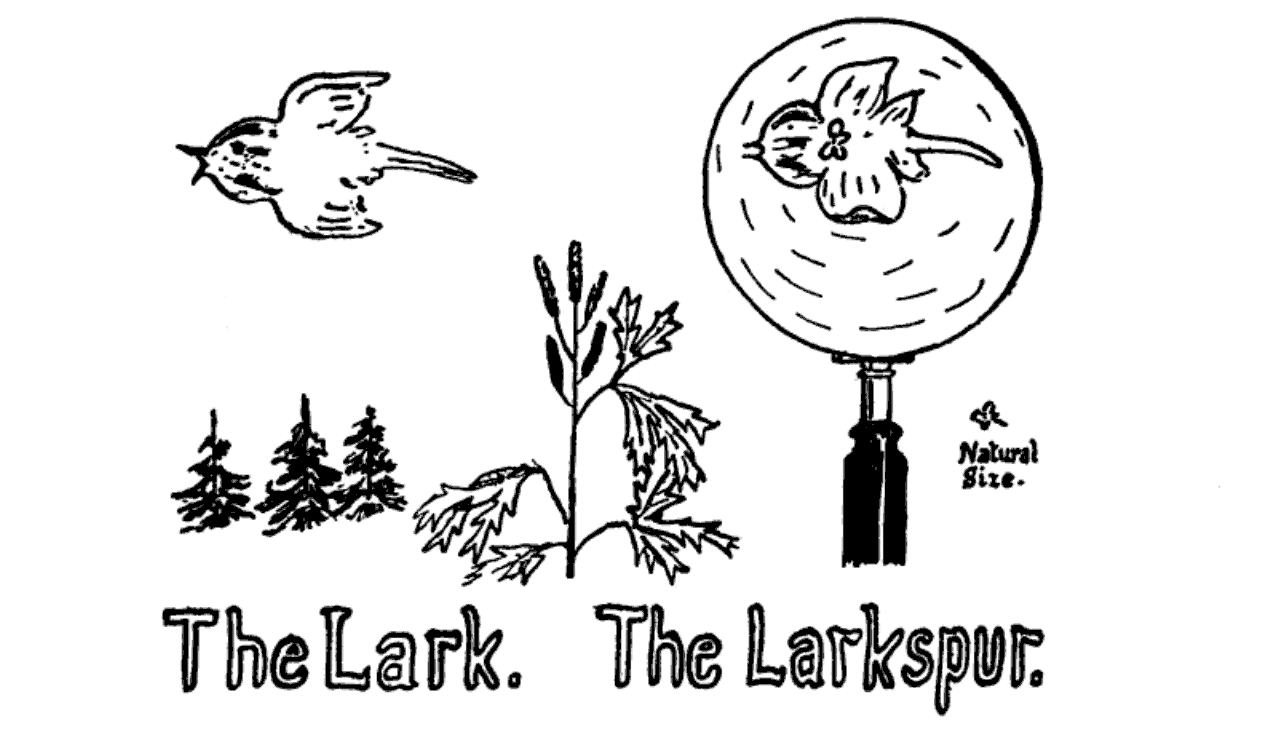
\includegraphics[width=1\textwidth]{f-p26.png}
\vspace{\onelineskip}
\begin{verse}\huge
The Larkspur's likeness to the Lark\\
Is surely worthy of remark,\\
Although to see it we require\\
The aid of a small magnifier,\\
Which circumstance of course implies,\\
Their difference is one of size.\\
\end{verse}

\chapter{The Puffin. Nuffin.}
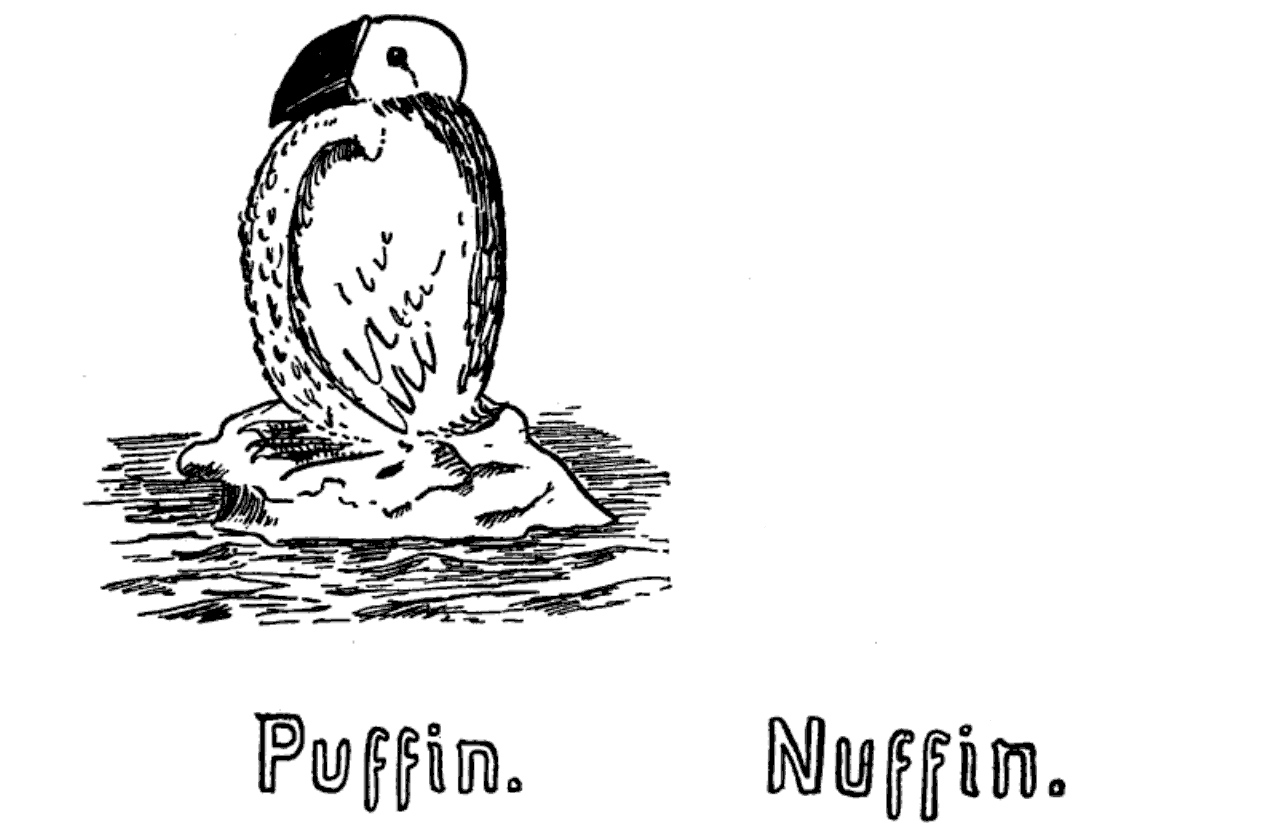
\includegraphics[width=1\textwidth]{f-p27.png}
\vspace{\onelineskip}
\begin{verse}\huge
Upon this cake of ice is perched\\
The paddle-footed Puffin:\\
To find his double we have searched,\\
But have discovered-Nuffin!\\
\end{verse}

\chapter{Author's Apology}
\PoemTitle*{\HUGE Author's Apology}
\begin{verse}\huge
Not every one is always able\\
To recognize a vegetable,\\
For some are guided by tradition,\\
While others use their intuition,\\
And even I make no pretense\\
Of having more than common sense;\\
Indeed these strange homologies\\
Are in most flornithologies,\\
And I have freely drawn upon\\
The works of Gray and Audubon,\\
Avoiding though the frequent blunders\\
Of those who study Nature's wonders.\\
\end{verse}

\end{document}
